\startfirstchapter{Motivation}
\label{chapter:introduction}

In this chapter I intend to provide some qualitative evidence to justify usefulness of grab and release actions.  
Grab and release actions were among the five most preferred hand interactions in a study done by Epps et al.\cite{Epps:2006:SHSUTGI} comparing preferences of user hand interactions for tabletop displays, and are a core component of many user interaction tasks. 
For example, users in Epps et al. suggested grab and release to perform actions such as cut, copy, moving icons or changing a slider.
I conducted a participatory design and brain storming sessions as well as a field study focused on how people use their hands while playing a board game. 
A summary of these studies will be presented here, because my choice of studying grab and release actions has been driven also by these studies.

\section{Backgammon Field Study}
Six individuals (three females and three males) volunteered to participate in a study that required them to play a game of backgammon against another participant.
The objective of the study was to find and classify hand actions performed by users while they play a board game. 
Two of the participants were completely new to the game, two of them had some experience but did not identify themselves as experts, and the other two were experts. 
Players were paired together based on the level of expertise that they reported when they were first approached.
\begin{figure}[h]
 \centering
 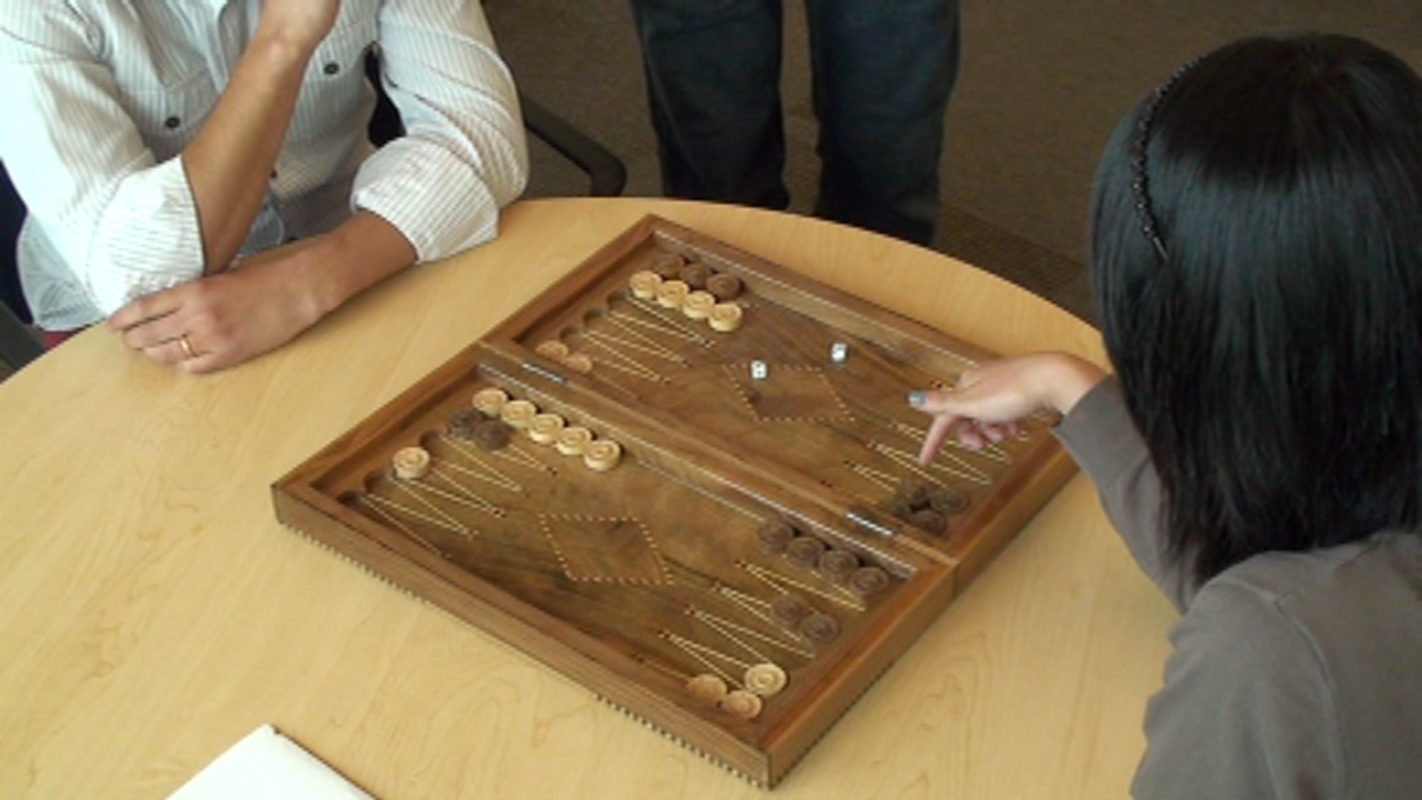
\includegraphics[type=pdf,ext=.pdf,read=.pdf,width=5in]{./img/backgammon_snapshot}
 \caption{ A snapshot of of one backgammon session }
 \label{fig:backgammon_snapshot}
\end{figure}
The videos of the study were manually coded to compile a list of actions and frequency of their occurrence in the videos.
Since the actions performed by users where almost always chained to achieve a task, I combined these actions whenever a common pattern was detected.
For instance when I observed grabbing of dice followed by throwing it I would classify that as one \textit{grab throw} action.
The actions on this list are compared in figure \ref{fig:backgammon_chart} grouped by the level of expertise of the participants.
\begin{figure}[h]
 \centering
 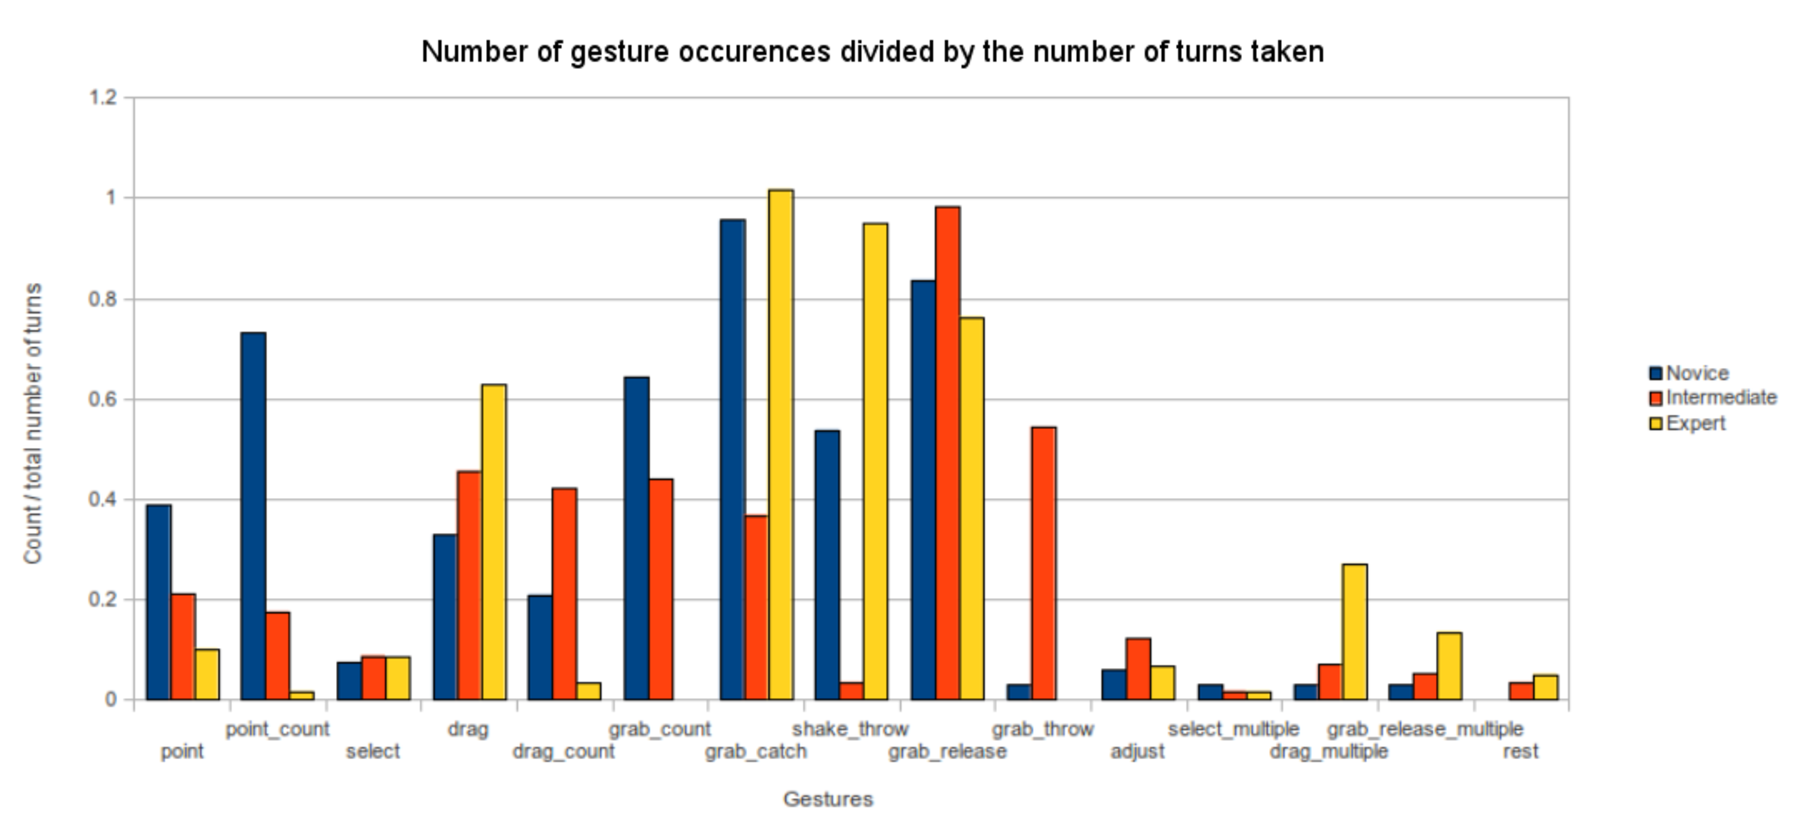
\includegraphics[type=pdf,ext=.pdf,read=.pdf,width=6in]{./img/backgammon_chart}
 \caption[Comparison of frequency of actions performed based on participant's level of expertise in the game of backgammon.]{
Comparison of frequency of actions performed based on participant's level of expertise in the game of backgammon.  
Since the number of turns in any given backgammon game could be different, the results are divided by the number of turns taken. }
 \label{fig:backgammon_chart}
\end{figure}
\subsection{Results}
Overall grab and release was the most popular gesture used by participants. 
Grab and catch and dragging are among other popular gestures in this game. 
Gestures such as point, point and count, and drag and count were performed more often by novice users. 
Those participants who identify themselves as experts in the game almost never used point and count or grab and count gestures. 
On the other hand gestures such as dragging, grab and release multiple, and drag multiple are more common among experts.

\subsection{Implications}
Many different variations of each single gesture were observed during the study. 
This suggest that a semantically single gesture for example “grab” can be done in different ways by different users, and even by the same user during her game. 
Therefore when developing a system to interpret and track hand pose and movement as a gesture, we should consider all of these variations.

Another implication of this study was that people can relate \textit{in the air} gestures to objects that are close to them. 
For instance when performing \textit{point count} gestures participants move their hand directly above game board to count the columns.
Therefore, I believe users can relate gestures directly above an interactive interface to the content of the interface. 
This result suggests that computer displays would be enriched if they were equipped with a sensing technology that could track the hand directly above the image that is displayed on them.

\section{Participatory Design Session}
Participatory design sessions consisted of researchers in our lab and invited participants who represent potential users of a near touch system. 
The session was started by providing users with some background information and motivation of this research.
It was explained to the users that I envision a system with which hand actions can be accurately detected in the area near the display screen.
Each participant was given a list of selected gestures which I prepared in advance based on the result of the backgammon field study. 
Next, the participants were asked to brainstorm on their own for five minutes about applications of the gestures from the list that they were given. 
After that I took approximately 40 minutes to discuss these ideas and brainstorm other gesture applications. 
The application area was intentionally not limited at this stage since I wanted to find out in what type of applications in general users may want to use these gestures.
Everyone was asked to use low fidelity prototyping tools that were provided to demonstrate their idea from this final list in front of a video camera so that the selected ideas could be expressed in a short video.
What I found from these sessions is that users can envision using near touch actions in various different application contexts.
From the list of actions that was provided to users, \textit{grab} and
\textit{release} generated the greatest number of application ideas.
Below is a list of some of the ideas that were proposed in these
sessions.
\begin{itemize}
 \item In a file management application, use \textit{grab} and \textit{release} in place of cut and paste to move files and folders. Keep one finger on a file or folder while \textit{grabbing} it with the other hand to obtain a copy of the item
 \item In a painting application, \textit{grab} a few colors from a palette and mix them by shaking your hand, then splash them on the screen by performing a release action
 \item In your home with multiple computing devices, \textit{grab} your news
feed from a desktop computer and \textit{release} it onto your tablet to
continue reading the news on the tablet device
 \item To organize a dashboard with several widgets, you can \textit{grab} a widget, move your hand above where you want it and \textit{release} it to its new location
 \item While playing a video game, in order to acquire an item such as a new weapon or a first aid kit you can just \textit{grab} it when you see it
 \item In a music player, perform a \textit{grab} action above the play-list to obtain it, then shake your hand to shuffle the music, and \textit{release} the play-list back down to start playing your music
\end{itemize}